	\documentclass[11pt]{article}
%Gummi|065|=)
%\title{\textbf{Welcome to Gummi 0.6.5}}

\title{\textbf{AIND Planning Project}}


 \renewcommand{\familydefault}{Hoefler}

\usepackage{amsmath}	
\usepackage{tikz}
\usepackage{xcolor}
\usepackage{float}
\usepackage{graphics}
\usepackage{graphicx}
\usepackage{wrapfig}
\usepackage{slashbox}
\usepackage{csvsimple}

\usetikzlibrary{shapes,arrows,chains}


\begin{document}

\maketitle

\newpage


\section{Uninformed Search Algorithms}

\subsection{breadth first search}
A search algorithm that searches the shallowest nodes in the tree first, excluding already explored states.
If a solution exists this algorithm will find it, though it may not be optimal.

\subsection{breadth first tree search}
Similar to breadth first this allows for repeated states.	
Not only could this solution create non optimum solutions there also exists the possibility of no solution being found as the algorithm falls into a cyclic search pattern dominating the search space, meaning that the problem space is not explorable with a feasible amount of computational power and/or storage space.

\subsection{depth first graph search}
Expanding the last expaned node until:
\begin{itemize}
	\item the goal is found
	\item there are no nodes left in current branch
	\item a previously explored state has been reached
\end{itemize} 
The limitation here on not exploring a previously explored space makes the algorithm efficient computationally but can prevent the algorithm from finding optimal solutions, it will not look for less expensive routes to the goal.

\subsection{depth first limited search}
Similar to depth first, but allowing for exploration of previously explored states. While this has the potential to find optimal solutions it may fall afoul of cycling through the same set of actions ad infinitum resulting in no solution being found even when one exists.

\subsection{greedy best first graph search}
Associating a cost with each action and expanding the action that is judged to be closest to the goal iff the state has not been explored already. This is reliant on the heuristic associated with the action being a good representation of closeness to the goal.

\subsection{uniform cost search}
Greedy best first graph search applying a uniform cost to all actions, effectively making a pseudo breadth first search, however the greatest difference is that uniform cost search does not stop immediately once the goal is found, instead examining other nodes at the goal found goal depth\cite{russell2005ai}, meaning it will produce the same result as breadth first but potentially less efficiently.\\

\textbf{*Note:} an optimum solution here is defined as minimizing the number of actions, and assumes that all actions have the same cost.

\section{A* Search}
A* is a best first search with the caveat it evaluates nodes within the search tree by minimizing the sum of the cost to reach a given node and the approximate distance from the node to the goal, it is both complete and optimal \cite{russell2005ai}.


\section{Planning Graph}
A planning graph is a useful tool that can be used to solve propositional problems. Breaking the problem down into alternating layers of states and actions. It can be used to estimate the number of steps between states and is polynomial in size, as an approximation, when a complete and exact tree would be exponential\cite{russell2005ai}. It should be noted that this is not a perfect tool, it only guarantees that if a goal state is not found before it levels off (where a state-action pair result in identical successive state-action pairs) then there is no solution. Even if a goal state is found all that can be said is that a solution \underline{may} exist.

\subsection{ignore preconditions}
This would be a heuristic that evaluates a node as the number of steps to achieve all goals while ignoring any preconditions.


\subsection{level sum}
Within a planning graph this would be the sum of the number of action levels required to achieve each goal in isolation.


\section{Uninformed Search Results}

\begin{figure}[H]
%	\centering
	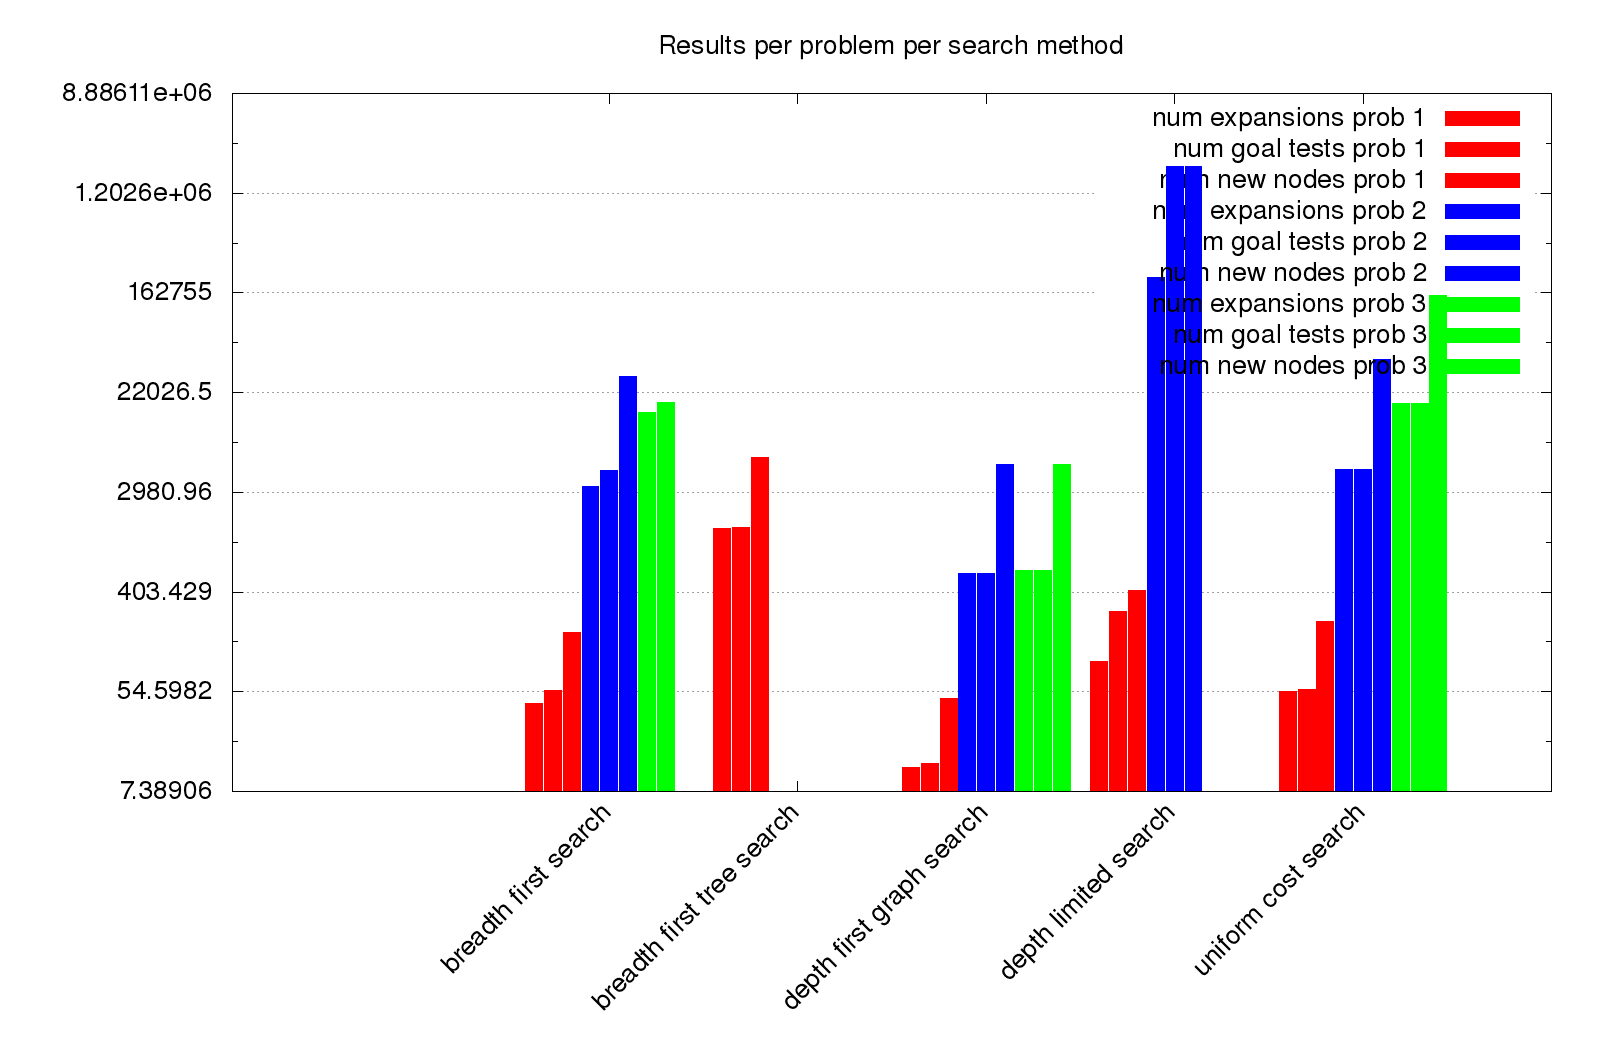
\includegraphics[scale=0.32]{results_summary.png}
	\caption{Results of each search method on each heuristic. The y axis is scaled to $log(e)$.
			 It should be noted that problems 2 and 3 were not solved by breadth first within reasonable time. and that problem 3 was not solved by depth limited in reasonable time.}
	\label{uninformed_results_summary}
\end{figure}

\begin{figure}[H]
	\begin{tabular}{|p{2cm}|| p{1.3cm} p{1.3cm} | p{1.3cm} p{1.3cm} | p{1.3cm} p{1.3cm} |} 
		\hline
		algorithm & p1 num steps & p1 runtime & p2 num steps & p2 runtime & p3 num steps & p3 runtime \\
		\hline
		\hline
		breadth first search & 6 & 0.0227 & 9 & 10.3 & 12 & 80.6  \\
		\hline
		breadth first tree search & 6 & 0.680 & N/A & N/A & N/A & N/A  \\
		\hline
		depth first graph search & 12 & 0.00605 & 575 & 2.71 & 596 & 2.94  \\
		\hline
		depth limited search & 50 & 0.06507 & 50 & 730 & N/A & N/A  \\
		\hline
		uniform cost search & 6 & 0.0263 & 9 & 8.64 & 12 & 36.5  \\
		\hline
		uniform cost search A* & 6 & 0.0306 & 9 & 8.84 & 12 & 38.6 \\
		\hline
		ignore precondition A* & 6 & 0.0287 & 9 & 3.04 & 12 & 11.6\\
		\hline
		level sum A* & 6 & 0.923 & 9 & 125 & 13 & 579 \\
		\hline
	\end{tabular}
	\caption{steps and runtime per problem, it is worth noting that runtime is an unreliable figure given that the system was under unrelated load during these tests.}
	\label{results_timestep}
\end{figure}

\subsection{Problem 1}

\textbf{Optimal uninformed solution:}
\begin{enumerate}
	\item Load(C2, P2, JFK)
	\item Load(C1, P1, SFO)
	\item Fly(P2, JFK, SFO)
	\item Unload(C2, P2, SFO)
	\item Fly(P1, SFO, JFK)
	\item Unload(C1, P1, JFK)
\end{enumerate}

The simplest of problems with least goals and constraints, it is solvable within 6 steps.

Given that planes start at the same locations as cargo, and there is one plane per unit of cargo, the problem can be solved in load, fly, unload for each piece of cargo.

Given this simplicity how do the different search algorithms fair against this challenge?

Figure \ref{results_timestep} shows that breadth first, breadth first tree, and uniform cost searches find the optimal solution and that depth first graph search and depth first limited search find non optimal solutions but with reduced runtime, though it should be noted that in terms of number of expansion, goal tests and new nodes depth first graph search is most efficient. 

\subsection{Problem 2}

\textbf{Optimal uninformed solution:}
\begin{enumerate}
	\item Load(C2, P2, JFK)
	\item Load(C1, P1, SFO)
	\item Load(C3, P3, ATL)
	\item Fly(P2, JFK, SFO)
	\item Unload(C2, P2, SFO)
	\item Fly(P1, SFO, JFK)
	\item Unload(C1, P1, JFK)
	\item Fly(P3, ATL, SFO)
	\item Unload(C3, P3, SFO)
\end{enumerate}

In contrast to problem one this has an added layer of complexity, but is similar in that planes start at the same location as cargo, and no cargo is at its associated goal. Given this the optimal number of steps is 9, as produced by breadth first and uniform cost search. The additional variables meant that breadth first tree search was not practical for this problem, the algorithm likely fell into a cycle of repetition undoing its actions not completing the search. While breadth first and uniform cost searches provided the optimum answers they took more expansions, goal tests and new nodes than depth first graph search. 575 steps from depth first search is far from the correct answer of 9 provided by by uniform cost and breadth first.

Depth limited search found a better answer than uniform cost, at 50 vs 575, however this was at the expense of many orders of magnitude more expansions, goal tests and new nodes. 

Breadth first tree search was unable to find a solution to this problem within a reasonable amount of time.


\subsection{Problem 3}

\textbf{Optimal uninformed solution:}
\begin{enumerate}
	\item Load(C2, P2, JFK)
	\item Load(C1, P1, SFO)
	\item Fly(P2, JFK, ORD)
	\item Load(C4, P2, ORD)
	\item Fly(P1, SFO, ATL)
	\item Load(C3, P1, ATL)
	\item Fly(P1, ATL, JFK)
	\item Unload(C1, P1, JFK)
	\item Unload(C3, P1, JFK)
	\item Fly(P2, ORD, SFO)
	\item Unload(C2, P2, SFO)
	\item Unload(C4, P2, SFO)
\end{enumerate}

A more complex problem in comparison to the previous two, 4 units of cargo and two planes. The optimum number of steps in this case is 12, requiring each plane to make additional trips to pick the cargo up and fly it to its destination.

Both breadth first tree and depth limited searches were unable to find a solution within a reasonable amount of time, likely falling into cycles of finding repeated states and the search space being impractically large respectively.

While the best performer in terms of time was depth first graph search, this produced the obviously non optimal number of steps as 596, more than an order of magnitude incorrect. In terms of which algorithm what better suited to this in terms of both getting the right answer most efficiently that would be breadth first. This is expected as uniform cost search is at its heart breadth first with additional work -- the same applied to all other problems.

\section{Planning Graph A* Search Results}
\begin{figure}[H]
%	\centering
	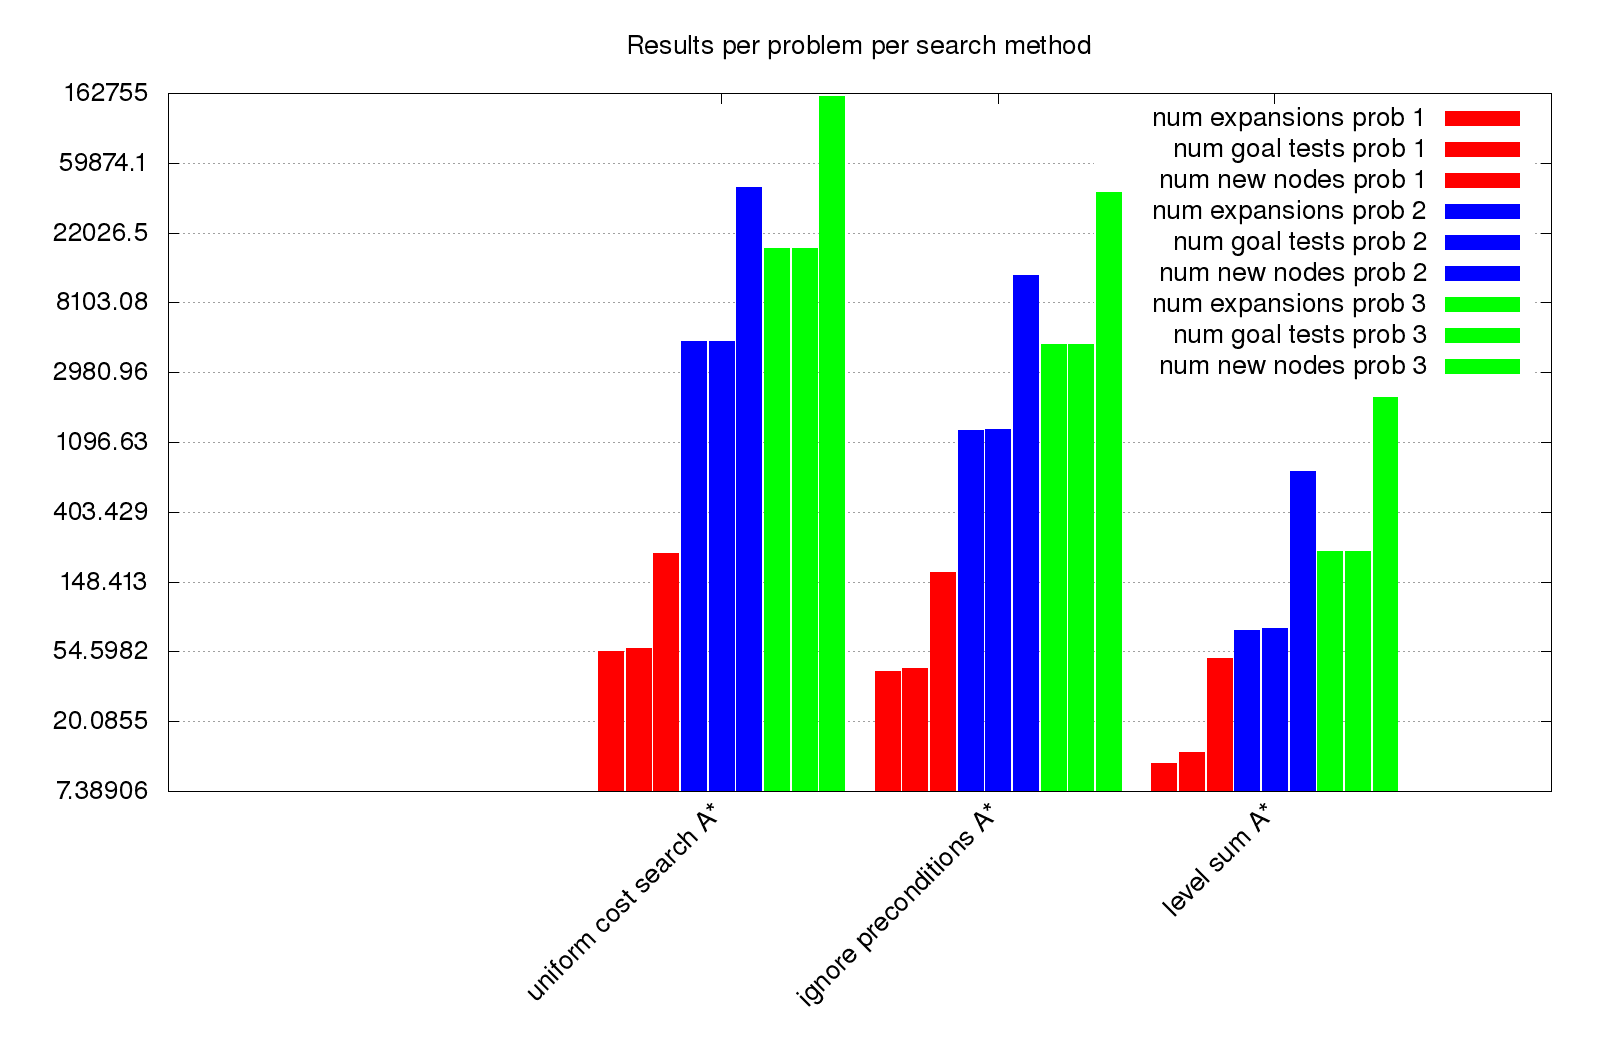
\includegraphics[scale=0.32]{pg_results_summary.png}
	\caption{Results of A* search method on each heuristic. The y axis is scaled to $log(e)$.}
	\label{a_star_results_summary}
\end{figure}

\begin{figure}[H]
%	\centering
	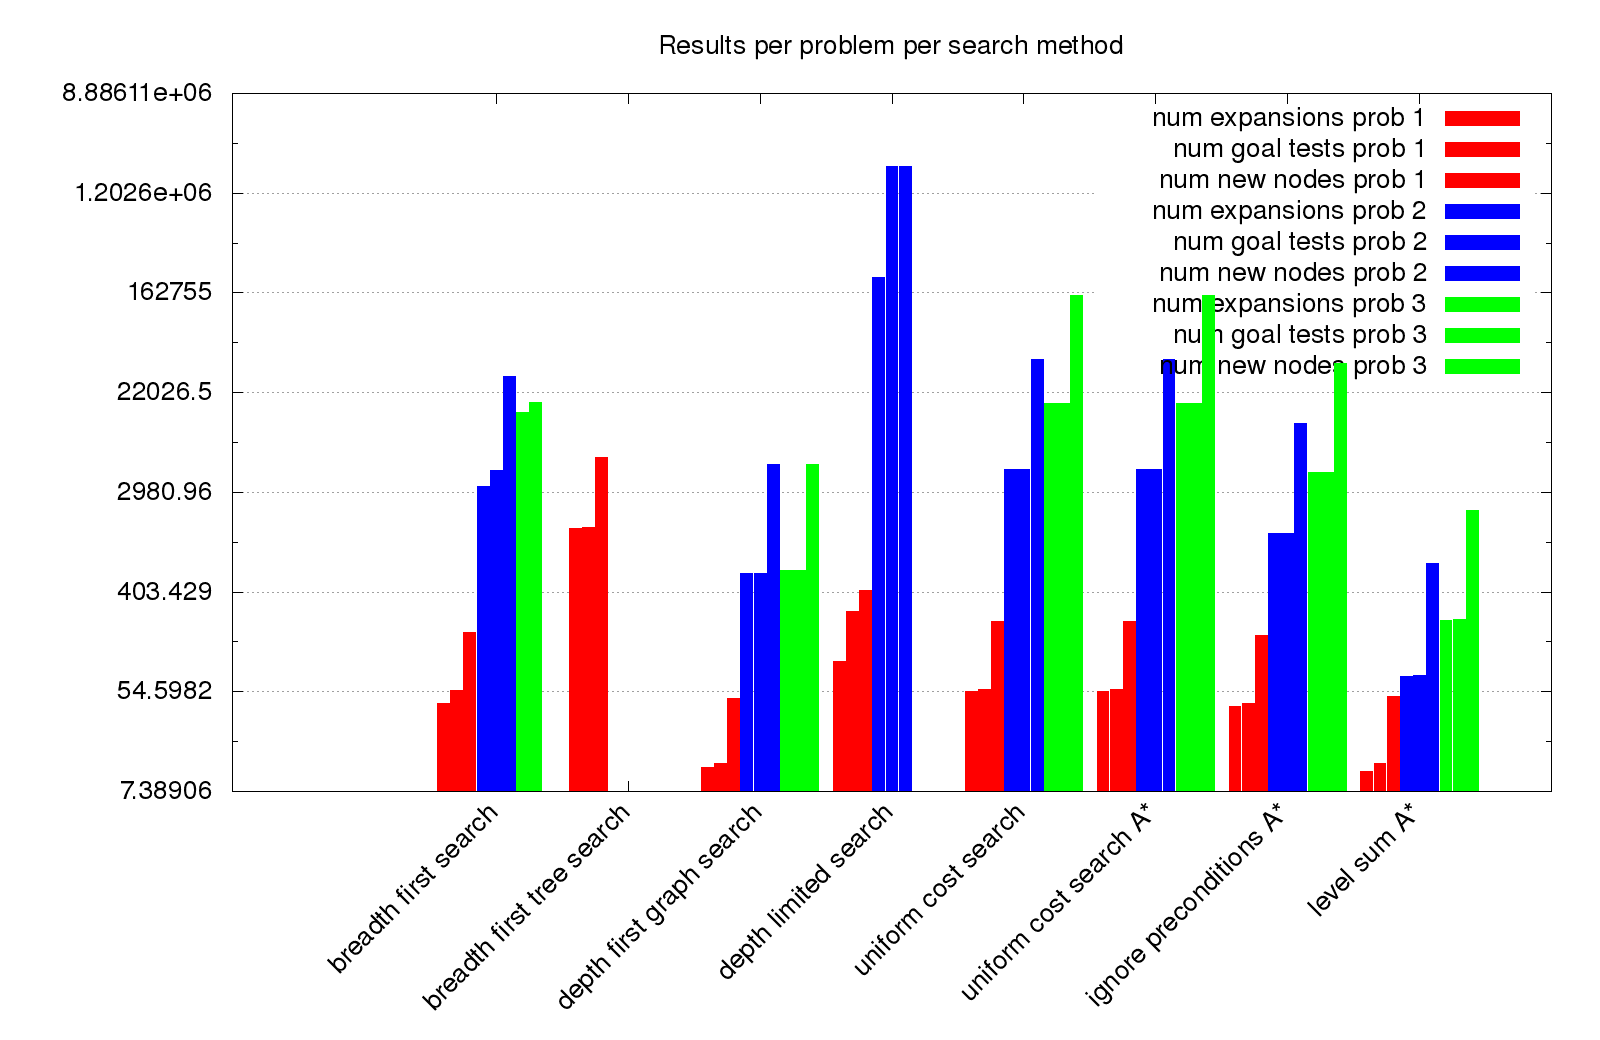
\includegraphics[scale=0.32]{complete_results_summary.png}
	\caption{Results of all search method on each heuristic. The y axis is scaled to $log(e)$.}
	\label{complete_results_summary}
\end{figure}

\subsection{Problem 1}
\textbf{Optimal A* solution:}
\begin{enumerate}
	\item Load(C1, P1, SFO)
	\item Load(C2, P2, JFK)
	\item Fly(P1, SFO, JFK)
	\item Fly(P2, JFK, SFO)
	\item Unload(C1, P1, JFK)
	\item Unload(C2, P2, SFO)
\end{enumerate}

As expected A* with uniform cost search is identical to  a uniform cost search. Both the ignore precondition heuristic and level sum heuristic achieved a goal state, both in less expansions than the other heuristics with level sum requiring the least expansions, goal tests and new nodes(excluding depth first which produced drastically incorrect results). However level sum took the longest.

\subsection{Problem 2}
\textbf{Optimal A* solution:}
\begin{enumerate}
	\item Load(C1, P1, SFO)
	\item Load(C2, P2, JFK)
	\item Load(C3, P3, ATL)
	\item Fly(P1, SFO, JFK)
	\item Fly(P2, JFK, SFO)
	\item Fly(P3, ATL, SFO)
	\item Unload(C1, P1, JFK)
	\item Unload(C2, P2, SFO)
	\item Unload(C3, P3, SFO)
\end{enumerate}

Again A* with uniform cost is no different from uniform cost. Level sum achieved the correct solution with the least expansions, goal tests and new nodes, however too far longer than other heuristics.

\subsection{Problem 3}
\textbf{Optimal A* solution:}
\begin{enumerate}
	\item Load(C1, P1, SFO)
	\item Fly(P1, SFO, ATL)
	\item Load(C3, P1, ATL)
	\item Fly(P1, ATL, JFK)
	\item Unload(C3, P1, JFK)
	\item Unload(C1, P1, JFK)
	\item Load(C2, P2, JFK)
	\item Fly(P2, JFK, ORD)
	\item Load(C4, P2, ORD)
	\item Fly(P2, ORD, SFO)
	\item Unload(C4, P2, SFO)
	\item Unload(C2, P2, SFO)
\end{enumerate}

Again identical results from uniform cost, A* or otherwise. Again level sum and ignore preconditions heuristics achieved solutions within the least number of expansions, goal tests and new nodes with level sum taking the longest. In this case level sum did not achieve an optimal solution, taking an extra step at 13 steps instead of 12.


*Note: all A* solutions presented above are optimal solutions

\section{Conclusion}
In terms of correctness and speed A* with ignore preconditions is the best search algorithm, being the fastest that achieves optimal results. Superficially level sum may appear to be one of the worst, despite achieving reasonable, not always optimal results, however with appropriate optimization of the algorithm it has the potential to strike a balance between correctness and speed.

The worst heuristic is breadth first tree search which fails to find solutions that are present, and taking significant time when it does. Even when it finds a solution it fails to provide an optimal one. Almost as bad is depth first limited search which is more likely to find a solution but will likely not be correct while also being computationally expensive. 

Whilst depth first graph search finds a solution it does not find optimal solutions, or solutions which are even reasonable.

\bibliography{refs.bib}
\bibliographystyle{plain}


\end{document}
